\subsection{A solução}

  Primeiramente\footnote{Mesmo sendo um jogo com regras, relativamente,
  simples, e uma aplicação com escopo bem limitado, este é um estudo que não
  se possa encerrar em 20 páginas, considerando a quantidade de código que
  pode vir a ser gerada. Também é necessário salientar que o contexto de
  automatizar um processo cujas regras já estão bem definidas apresenta
  privilégios não compartilhados em uma situação mais próxima do real, mas
  servem bem aos critérios didáticos pretendidos.}
  usamos uma técnica chamada
  \emph{Mapeamento de Histórias de Usuário}\footnote{\cite{Patton2014}}
  para identificar fluxos completos de uso, conforme
  \textbf{Figura \ref{fig:fluxogeral}}. Essa técnica permite não só definir
  todas as histórias que se deseja ver implementadas mas, também, aquelas
  que agregam maior valor ao resultado, possibilitando a delimitação de um
  produto mínimo viável (MVP) que atenda às necessidades daquele e, ainda,
  gerenciem os riscos de construir uma solução pormenorizada, antes mesmo de
  validar algumas hipóteses.

  \begin{figure}[h]
    \centering
    \caption{Mapeamento de Histórias de Usuário}
    \efbox{
      \makebox[\textwidth]{
        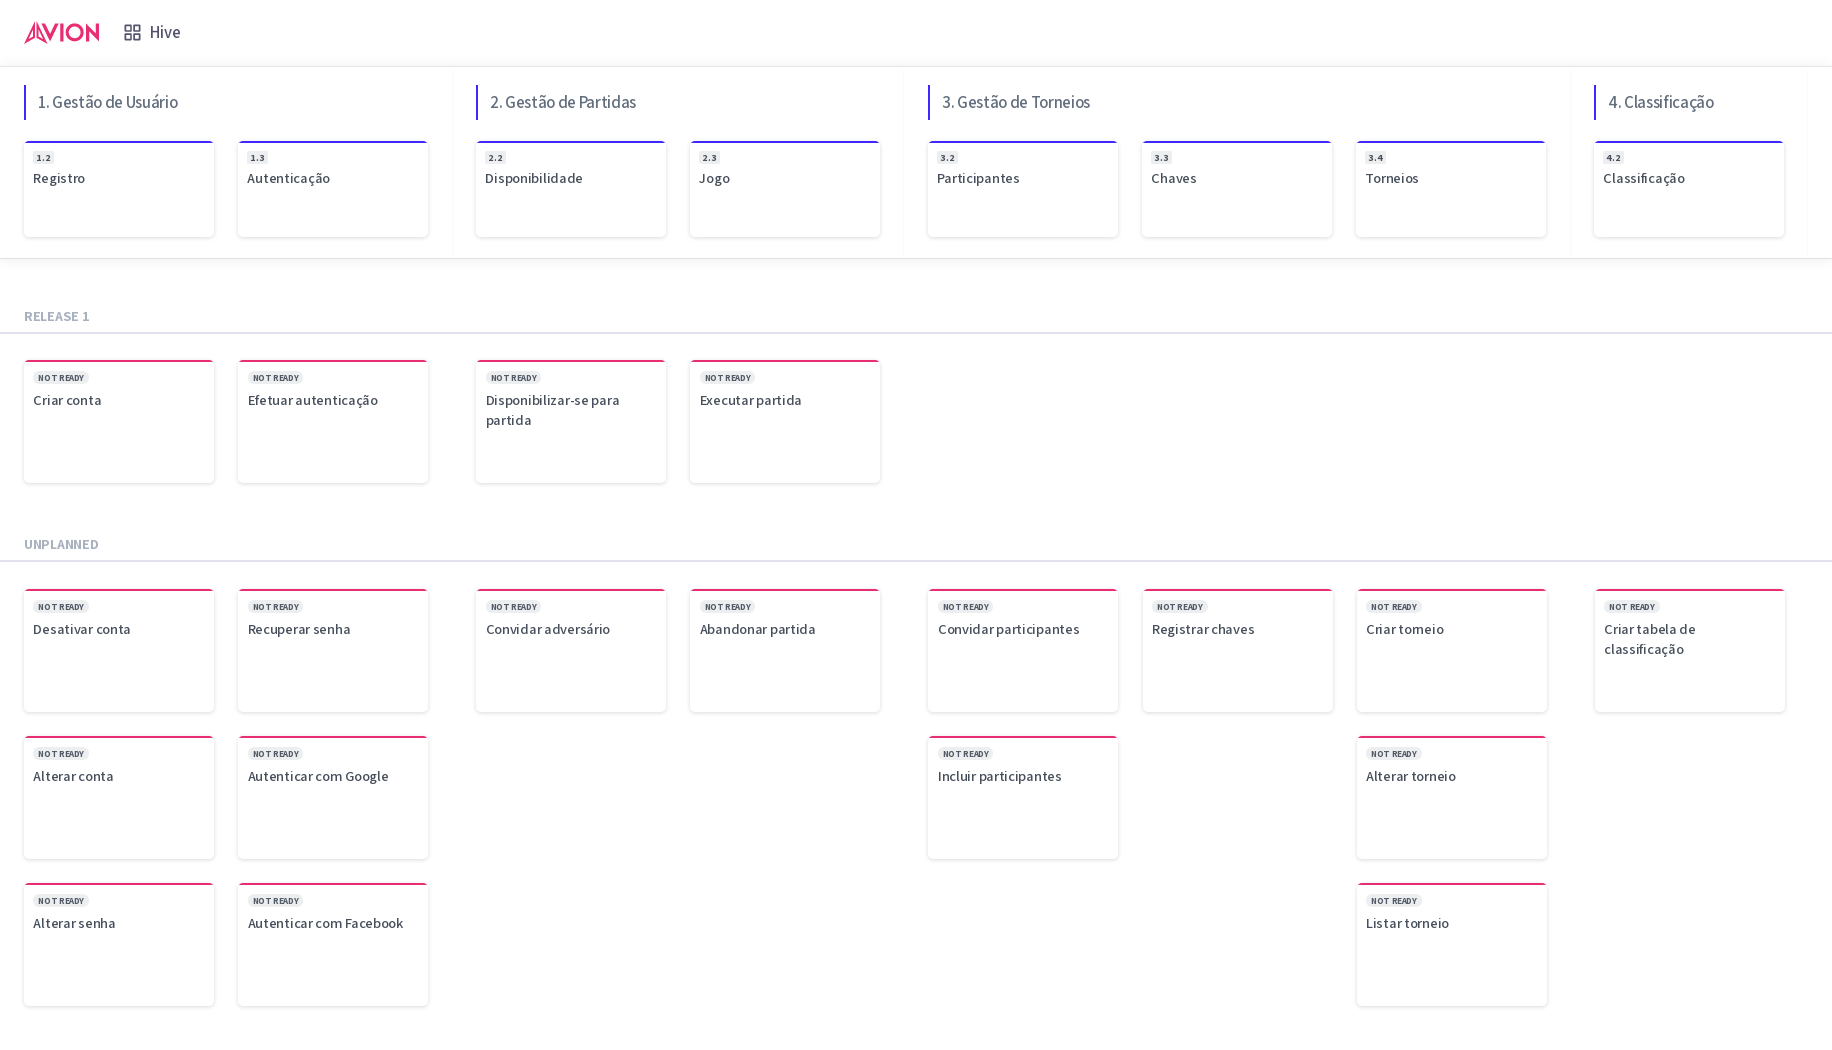
\includegraphics[width=\textwidth]{user-stories-mapping}
      }
    }
    Fonte: Próprio autor\footnotemark
    \label{fig:fluxogeral}
  \end{figure}
  \footnotetext{Criado usando \url{https://app.avion.io}}

  Assim, podemos perceber que quatro funcionalidades são essenciais para o
  MVP: \emph{Criar conta}; \emph{Efetuar autenticação};
  \emph{Disponibilizar-se para partida}; e, \emph{Executar partida}.

  Um exercício bem simples para saber se uma história é muito grande, ou
  muito pequena, é elencar os cenários vinculados. Parâmetros comumente
  usados são não menores que 2 e não maiores que 7. Para aquelas, os
  cenários listados na \textbf{Figura \ref{fig:cenarios-das-historias}}
  foram levantados.

  \begin{figure}[h]
    \centering
    \caption{Cenários das histórias}
    \lstinputlisting[numbers=none]{Cenarios.txt}
    Fonte: Próprio autor
    \label{fig:cenarios-das-historias}
  \end{figure}

  O que sugere uma quebra da história \emph{Executar partida} em pelo menos
  outras três, como observavél na \textbf{Figura \ref{fig:executar-partida}}.

  \begin{figure}[h]
    \centering
    \caption{Quebra da história \emph{Executar partida}}
    \lstinputlisting[numbers=none]{ExecutarPartida.txt}
    Fonte: Próprio autor
    \label{fig:executar-partida}
  \end{figure}

  De posse desses subsídios, faz-se mister escolher um cenário, levando em
  consideração a simplicidade e completude. Explique-se, um que seja simples
  o suficiente para não criar um entrave logo no início dos trabalhos mas
  que ainda seja capaz de exercitar o maior número de componentes da
  estrutura da aplicação. Sendo assim, selecionamos
  \emph{Propor partida/Com adversário disponível}. O movimento seguinte é
  detalhar este, de onde se extrai os passos observáveis na \textbf{Figura
  \ref{fig:passos-primeiro-cenario-escolhido}}.

  \begin{figure}[h]
    \centering
    \caption{Detalhamento do cenário escolhido}
    \lstinputlisting[numbers=none]{PassosPrimeiroCenarioEscolhido.txt}
    Fonte: Próprio autor\footnotemark
    \label{fig:passos-primeiro-cenario-escolhido}
  \end{figure}
  \footnotetext{Aqui fizemos uso da do modelo criado por
  \citeonline{North2006} que ficou conhecido como \emph{Behaviour Driven
  Development} (\emph{Desenvolvimento guiado por comportamento}, em tradução
  livre). Mais precisamente, a síntaxe adotada pelo framework Cucumber,
  \emph{Gherkin}.}

  Importante notar a linguagem utilizada, que não faz qualquer referência as
  tecnologias que dão suporte a solução mas, tão somente, expressão o
  linguajar dos interessados\footnote{Batizado por
  \citeonline[pág. 24]{
  Evans2003} de \emph{Ubiquitous Language} (Linguagem Ubíqua, em tradução
  livre).}.

  As primeiras experiências são mais difíceis, mas vale o esforço. Uma dica
  é usar o que \citeonline[págs. 142 e 226]{Abelson1996} chamam de \emph{
  wishful thinking}\footnote{\emph{Pensamento positivo, ou, mais
  específico, Programação por desejo}, em tradução livre.} - ou o que,
  \citeonline[págs. 136-146]{Astels2002}, chama de \emph{Código com intenção}
  - que, na prática, significa escrever um teste como se a funcionalidade
  alvo já existisse. Isso mantém o foco em \emph{o quê} o sistema deve fazer
  em contraposição a \emph{como} ele o fará. Pode parecer uma diferença
  desprezável, mas o tempo (perdido corrigindo testes frágeis) mostrará que
  há um abismo inteiro na forma como esta solução estará aberta à gradual
  evolução (fora o efeito nocivo que isso tem sobre o moral do desenvolvedor).

